
\documentclass[submit,techrep,noauthor]{ipsj}


\usepackage[dvipdfmx]{graphicx}
\usepackage{latexsym}
\usepackage{url}
\usepackage{xcolor}
\usepackage{listings}
\usepackage{amsmath,amssymb}


% コード例を載せるためのあれこれ
\definecolor{lightred}{RGB}{255,230,230}
\definecolor{lightgreen}{RGB}{230,255,230}

\lstset{
basicstyle=\small\ttfamily,
abovecaptionskip=0pt,
captionpos=b,
frame=tb,
framexleftmargin=2em,
numbers=left,
numberstyle={\scriptsize},
xleftmargin=\parindent,
escapechar=| 
}

%ListingのキャプションがFigureになってしまうのをListingに直すコマンド
\usepackage{caption}
\makeatletter
\let\MYcaption\@makecaption
\makeatother
\usepackage{caption}
\makeatletter
\let\@makecaption\MYcaption
\makeatother

\newcommand{\todo}[1]{\colorbox{yellow}{{\bf TODO}:}{\color{red} {\textbf{[#1]}}}}
\newcommand{\ihara}[1]{\colorbox{green}{{\bf IHARA}:}{\color{blue} {\textbf{[#1]}}}}

\def\Underline{\setbox0\hbox\bgroup\let\\\endUnderline}
\def\endUnderline{\vphantom{y}\egroup\smash{\underline{\box0}}\\}
\def\|{\verb|}
%

\def\Underline{\setbox0\hbox\bgroup\let\\\endUnderline}
\def\endUnderline{\vphantom{y}\egroup\smash{\underline{\box0}}\\}
\def\|{\verb|}

\begin{document}


\title{CodeQLを用いた繰り返し処理を含む
\\
低速コードパターン検出手法
}

\affiliate{IPSJ}{和歌山大学\\
Wakayama University}

\author{野口 隼杜}{Noguchi Hayato}{IPSJ}[s276185@wakayama-u.ac.jp]
\author{野口 朋弥}{Noguchi Tomoya}{IPSJ}[s266227@wakayama-u.ac.jp]
\author{伊原 彰紀}{Ihara Akinori}{IPSJ}[ihara@wakayama-u.ac.jp]

\begin{abstract}
ソフトウェアの性能効率化は品質に直結する重要な課題であるが,ソースコード中に複数検出される性能ボトルネックの中から修正箇所を選定することは,開発者の経験に大きく依存している.また,プロファイラなどの動的解析ツールは,プログラムがある程度実装された後にしか適用できず,開発早期での性能改善作業を困難にしている.本研究では,この課題に対し,CodeQLによる静的解析を活用した繰り返し処理を含む低速コードパターンの早期検出手法を提案する.まず,プログラムの実行速度を比較するマイクロベンチマークを利用し,実行速度に差のある実装対から低速の原因となるコードパターンを作成する.次に,このコードパターンを基に,静的解析エンジンであるCodeQLのためのカスタムクエリを作成し,ソースコード中から該当する低速パターンを開発の早期段階で検出する.さらに,検出された箇所の依存関係を解析することで,修正が全体に与える影響や修正の優先度を推定する可能性についても言及し、より効果的な高速化修正候補の特定を目指す.ケーススタディを通じて,作成するコードパターンによる検出精度を評価するとともに,マイクロベンチマークを起点とする早期の性能改善アプローチの有用性について考察する.
\end{abstract}


\maketitle

%1
\section{はじめに}

 ソフトウェアの性能効率性は,ユーザ体験や運用コスト,さらにはシステム全体の品質に直結する重要な要素である.ここで,性能効率性の向上には,計算機能力やシステム設計の改善だけではなく,部分的なソースコードの最適化を積み重ねることで実現される場合も多い.例として,Webアプリケーション開発では,数行のコード修正による最適化を行っており,結果としてプログラムの実行時間が25%から70%高速化している\cite{jsRefac}

性能効率性向上のためのプログラム変更については,実装が進行するにつれて,複雑になりやすいことが定量的に明らかにされている\cite{complicate}.また,このプログラム変更においては,保守性や可読性など,他のプログラム品質に否定的な影響を与えることもあり\cite{negative},プログラムが表現できる多様な実装方法の中から代替する最適な実装を選択するために,開発者に広範な知識や技量を求める.そのため,ソフトウェアの性能効率性を,実装途中の早期の段階で見積もり,性能低下の原因箇所を検出することで,性能効率性の改善におけるコストや否定的な影響を小さくできることが考えられる. 

一般的に,ソフトウェアの性能効率性を評価する方法として,プロファイラなどの動的解析ツールが広く用いられている.これらのツールは,実行時の関数呼び出しやリソース使用状況を精緻に観測し,性能低下の発見,および原因箇所の特定を可能にしている.しかし,動的解析ツールによる性能効率性の評価は,最低限の機能が実行できるまで実装が進んだ状態でなければ適用することができないため,開発初期段階において,性能効率性の評価を行うことは難しい.

ここで,実装途中においても,部分的な性能を定量的に評価する手法として,マイクロベンチマークが用いられている.マイクロベンチマークは特定のコード片に対して実行時間を測定することで局所的な性能差を把握できる.JavaScriptでは,マイクロベンチマーク共有サービスとして JsPerf\footnote{\url{https://jsperf.app/}}やMeasureThat.net\footnote{\url{https://measurethat.net/}}がある.これらのサービスでは,ブラウザ上でマイクロベンチマークの実行環境を提供しており,比較したいJavaScriptプログラムの対を作成し,それらを実行することで,実行速度の測定および比較ができる.また,作成したプログラム対は保存され,すべてのユーザに公開されることで,プログラム対とその結果を共有することができる.開発者はこれらのサービスやプログラムセットを活用して最適な実装方法を検討することができる.

しかし,マイクロベンチマークをどう設計するか,マイクロベンチマークの結果をどう解釈するかは,性能効率性向上のためのプログラム変更と同様に,開発者の技量に依るところが大きい.さらに,どの箇所を対象にマイクロベンチマークの結果を適用すべきかを判断するには,事前に潜在的な低速箇所を特定する必要がある.複数の性能問題が存在する場合には,これらに加えて,どの箇所を優先的に修正すべきかの判断も必要となるが,プログラム全体の依存関係や構造が大きく影響するため,効率的な性能改善作業を体系的に行うことは容易ではなく,マイクロベンチマークの利用における課題となっている.

これらの課題を踏まえると,性能効率性の向上を効率よく行うためには,マイクロベンチマークによって得られる局所的な性能知見を,ソースコード全体に適用可能な形で活用し,開発初期から性能上のリスクを検出することが重要である.本研究では,マイクロベンチマーク共有サービスで提供されるマイクロベンチマークを利用し,プログラム実装対の構造から低速コードパターンを抽出する.これを利用し,静的解析エンジンであるCodeQL\footnote{\url{https://codeql.github.com/}}\cite{ql}を用いて,ソースコード中の類似パターンを早期に検出する手法を提案する.加えて,検出された箇所に対して依存関係を解析することで,修正がプログラム全体に与える影響や修正の優先度を推定する可能性についても検討する.これにより,動的解析に依存せずに潜在的な性能ボトルネックを実装初期段階から特定し,修正効果の高い箇所を効率的に見出すことを目指す.

続く\ref{sec2:format}章では,本研究で利用するマイクロベンチマーク共有サービスにおけるマイクロベンチマークの特徴に触れ,キーアイデアを示す.\ref{sec3:format}章 では,本研究の提案手法を述べ, \ref{sec4:format}章において,ケーススタディの結果について述べる. \ref{sec5:format}章で考察を行い,\ref{sec6:format}章で本研究における妥当性の脅威を述べた上で,\ref{sec7:format}章で総括する. 


%2
\section{マイクロベンチマークに基づく性能ボトルネック検出}
\label{sec2:format}


%2.1
\subsection{マイクロベンチマーク共有サービスにおける実装対}

本研究では,大森ら\cite{omori}が作成した,マイクロベンチマーク共有サービスjsPerfにおける,実行速度に有意差があり,外的振る舞いが等しいことが検証された実装対29,809件を利用する.以降,これらの実装対をマイクロベンチマーク実装対とし,各実装対において実行時間が長いコードを低速コード,実行時間が短いコードを高速コードとする.
マイクロベンチマーク実装対は,同一の機能を異なる方法で実装した非常に短いコードの対によって構成されており,データ構造や制御構文,使用するメソッドの選択などに多様性が見られる.これらの実装対を目視調査した結果,実装対の両方もしくは片方に繰り返し処理を含むものが多く存在することが確認された.特に,巨大な配列や長大な繰り返し処理を用いて性能差を強調する実装対や,繰り返し処理自体の違いによって実行時間に差が生まれる実装対など,複数の傾向が確認された.


%2.2
\subsection{繰り返し処理を含むマイクロベンチマーク実装対}
\label{section2.2}

このような観察結果から,本研究ではマイクロベンチマーク実装対に対して繰り返し処理構造に着目した特徴分析を行うこととした.対象とする繰り返し処理は,JavaScriptにおける for,for-of,for-in,while,および do-while 構文である.

% \todo{図1で示すように} 繰り返し処理を含む実装対が全体の約43%(12,948対)存在する.

分析にあたっては,各実装対のソースコードを GumTree \cite{gumtree}により抽象構文木へと変換し,実装対の抽象構文木間の差分解析を行った.差分解析の結果に対して,(1) 差分が直接繰り返し処理構造を含むか,および (2) 差分ノードの構造的な親要素に繰り返し処理が含まれるかを確認事項とし,繰り返し処理に関連する差分要素として収集した.抽出された箇所に応じて目視で確認を行い,実装対の構造的特徴および性能差との関係を整理した.
この分析の結果,マイクロベンチマーク実装対には繰り返し処理について,いくつかのパターンが存在することが明らかとなった.Listing~\ref{diff-inloop},Listing~\ref{diff-loop},Listing~\ref{diff-method}に,特徴となる部分について示す.

Listing~\ref{diff-inloop}は,それぞれfor文内で concat メソッド, push メソッドを用いている実装対である.これは,繰り返しの構造は一致しているが,繰り返し内部で実行する処理が異なるパターンである.
%----------------------------------
\begin{lstlisting}[caption=Pairs with differences within the loop, label=diff-inloop, captionpos=t]
// slow
for (var VAR_2 = 0; VAR_2 < 5000; VAR_2++)
    VAR_1 = VAR_1.concat([\"1\", \"2\"]);

// fast
for (var VAR_2 = 0; VAR_2 < 5000; VAR_2++)
    VAR_1.push(\"1\", \"2\");
\end{lstlisting}
%----------------------------------

Listing~\ref{diff-loop}は,それぞれ,for-in文を用いて配列の全要素にアクセスする実装と,同様の処理をwhile文で実装したものである.ここで示すパターンは実行時間の差が,繰り返し処理自体の違いに起因するパターンである.
%----------------------------------
\begin{lstlisting}[caption=Pairs with loop differences, label=diff-loop, captionpos=t]
// slow
for (var VAR_2 in VAR_1) {
    VAR_1[VAR_2];
}

// fast
var VAR_3 = 0;
while (VAR_3 < VAR_1.length) {
    VAR_1[VAR_3];
    VAR_3++;
}
\end{lstlisting}
%----------------------------------

Listing~\ref{diff-method}は,繰り返し処理をforEachメソッドで実装したものとfor-of文で実装したものである.これは,メソッドによる処理とそれに代替する繰り返し処理について比較したパターンである.
%----------------------------------
\begin{lstlisting}[caption=Pairs of Method and alternative loop, label=diff-method, captionpos=t]
// slow
var VAR_5 = new Set(VAR_2);
VAR_5.forEach(VAR_6 => {});

// fast
for (let VAR_7 of VAR_2) {}
\end{lstlisting}
%----------------------------------

これらの結果から,マイクロベンチマーク実装対には繰り返し処理の構造および繰り返し内部の操作内容の違いが性能差の主な要因として存在することが確認された.本研究では,このような繰り返し処理に関する差分構造を低速コードの特徴として抽出し,次章で述べる低速コードパターンの抽出および静的検出に利用する.


%2.3
\subsection{関連研究}

Selakovic ら\cite{jsRefac}は,JavaScript プロジェクトにおいて,開発者が高速化のために行ったリファクタリングを調査した.その結果,開発者は10行程度の小さい範囲の修正によって高速化への対処を行なっていることを明らかにした.この結果は,マイクロベンチマーク実装対に見られる,短いコードの高速化への利用可能性を示すものとして,本研究の動機づけとなっている.また,\cite{jsRefac}は,JavaScript プロジェクトの解析によって 10 件の頻出する高速化改良パターンを作成している.この改良パターンを用いた自動修正は一定の高速化効果を示しているが,システム上で効果的な修正箇所はどこかについては議論していない.

Turcotte ら\cite{DrAsync}は,JavaScript 言語における非同期処理に注目した性能アンチパターンを定義し,静的解析エンジンであるCodeQL\cite{ql}を利用したアンチパターンの検出と,動的解析を利用したパフォーマンスの監視を組み合わせ,修正可能な性能アンチパターンの検出を行った.本研究の静的解析による低速コードパターンの検出はこれに着想を得ている.

大森ら\cite{omori}は,マイクロベンチマーク共有サービスで公開される実行速度が向上するプログラムを収集し,これをデータセットとして大規模な言語学習モデルをファインチューニングすることで,実行を高速化するプログラムに自動リファクタリングするモデルを作成した.この結果,マイクロベンチマーク共有サービス上のプログラムに対しては,ChatGPT-4o より約3倍のリファクタリングに成功している.しかし,\cite{jsRefac}と同様,効果的な修正箇所についての議論はない.
 
本研究では,繰り返し処理に注目し,マイクロベンチマーク実装対における低速コードから構造的差分に基づいて低速コードパターンを抽出し,静的解析を用いて,性能ボトルネックの早期検出を行うとともに,プログラム上の依存関係を用いた,効果的な修正箇所の推定について議論する.


%3
\section{CodeQLクエリによる低速コードパターン検出手法}
\label{sec3:format}

%----------------------
\begin{figure*}[t]
    \centering
    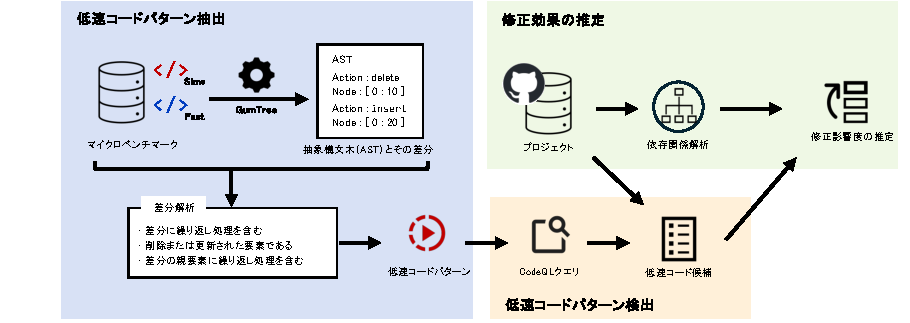
\includegraphics[width=1.0\linewidth]{./Noguchi_fig/approach_abst.pdf}
    \caption{本研究の全体像}
    \label{fig:Approach}
\end{figure*}
%----------------------

図\ref{fig:Approach}に,本研究で提案する手法の概略図を示す.本研究では,マイクロベンチマーク実装対より,低速コードの特徴を実装対の構造的差分から抽出し,低速コードパターンを作成する.作成したパターンをもとに静的解析エンジンCodeQL\cite{ql}を用いて,ソースコード中の低速コードを静的に検出する手法を提案する.また,検出結果について,修正効果の高い箇所をプログラム中の依存関係の数から推定する.以降でその詳細を述べる.


%3.1
\subsection{低速コードパターンの抽出}

\ref{section2.2} 節で述べたように,マイクロベンチマーク実装対において,繰り返し処理の構造および繰り返し内部の操作内容の違いが性能差の主な要因として存在することを確認した.したがって,本節では,繰り返し処理に注目して低速コードに特有の構造的特徴の抽出を行う.

\ref{section2.2} 節において収集した,繰り返し処理に関連する差分要素について,まず,低速コードから高速コードへのリファクタリングとした時に,GumTree\cite{gumtree} が削除または更新として検出したノードを取得する.これらのノードは,低速コードにのみ含まれる実装方法であり,対応する高速コードに対して,低速コード特有の処理構造を示すものであるため,低速コードパターンの候補とする.次に,取得したノードにおいて,使用されているメソッド呼び出しや配列・オブジェクト操作の形態および,それらの位置情報をもとに,低速コードパターンを特定する.


%3.2
\subsection{低速コードパターンの検出}

前節で抽出した低速コードパターンをもとに,本節では,ソースコード中に含まれる低速コードを静的に検出する手法について述べる.本研究では,\cite{DrAsync}に着想を得て,低速コードパターンを検出するための静的解析ツールとして CodeQL\cite{ql} を用いる.CodeQLは,GitHub が開発した,主にセキュリティ検査を自動化する目的で開発されたコード分析基盤であり,プログラムから抽象構文木の構築とデータフローの抽出を行い,それらをデータベースとして保持する.このデータベースに対して,SQL に類似したクエリ言語を用いて検索を行うことで,特定の構造や振る舞いを持つコード断片を効率的に抽出できる.

前節で作成した低速コードパターンをもとに,CodeQL において対応するカスタムクエリを作成し,ソースコード内で同様の構造を持つ箇所を検出する.カスタムクエリでは,低速コードパターンと一致する構文構造を抽出するよう,ASTノードの種類や親子関係を条件として指定する.クエリの作成にあたっては,マイクロベンチマーク実装対に適用し,その検出精度を検証するとともに,元となった低速パターンを含む低速コードを検出できるよう調整を行った.また,それ以外で検出された低速コードについても,目視で確認し,クエリの妥当性を検証した.最終的に作成したクエリを,元となった実装対とともに\todo{図}に示し,ケーススタディにおける低速コードパターンの検出に利用する.なお,次節で述べる関数の依存関係の解析を通して修正候補における効果を推定するため,本研究では,クエリによる検出単位を関数とし,特定の低速コードパターンを含む関数の検出を行う.


%3.3
\subsection{依存関係に基づく修正効果の推定}
低速コードパターンの検出結果について,検出された全ての箇所がシステム全体の性能改善に寄与するとは限らない.これは,本研究で用いたマイクロベンチマークが,特定のコード断片における処理性能を定量的に評価するためのものであり,部分的な性能差がそのままシステム全体の性能に直結するとは限らないためである.そのため,検出された低速コードパターンを含むソースコードのうち,「修正効果の高い箇所」を推定することで,低速コードパターンの検出結果を効果的に利用することができる.

ここで,修正効果について,単純に一回の処理が高速化されるだけでなく,その処理が繰り返し呼び出される頻度や,他の関数に与える影響の大きさが修正効果を決定する一因となる.つまり,実行頻度や依存度の高い関数ほど,その改善によって波及効果が大きいと考えられる.このことから,本研究では,関数の依存関係に基づいて修正効果を推定する.

(1)関数依存関係の構築

関数間の依存関係を構築するために,本研究では JavaScript/TypeScript の静的解析ツールである Jelly\todo{リンク} を用いる.Jelly は,ソースコードを静的に解析し,関数呼び出しを基点とするコールグラフを構築できるツールである.Jelly により得られたコールグラフをもとに,各関数がどの関数を呼び出しているか,およびどの関数から呼び出されているかを抽出する.

(2)修正効果の推定

構築された関数依存関係をもとに,低速コードパターンを含む関数の修正効果を次の指標で評価する.注目する関数$ f_i $に対して,その関数が呼び出している関数の数(出次数)および他の関数から呼び出されている数(入次数)をそれぞれ算出する.これらの値の合計を関数の依存度とし,次式で表す:

\begin{equation}
D(f_i) = \mathrm{out\_deg}(f_i) + \mathrm{in\_deg}(f_i)
\end{equation}

ここで,$ out\_deg(f_i) $は関数$ f_i $が呼び出している関数の数,$ in\_deg(f_i) $は関数$ f_i $がは他の関数から呼び出されている数を示す.前者が大きい場合,その関数の高速化は内部で呼び出している複数の処理を通じてプログラム全体の処理効率を高める効果があると考えられる.一方,後者が大きい場合,関数が多くの他関数から利用されており,その高速化がシステム全体に波及する可能性が高いことを意味する.したがって,本研究では,低速コードパターンを含む関数に対して$ D(f_i) $の値を算出し,これを修正効果の推定指標として用いる.依存度の高い関数ほど修正効果が大きいとみなし,修正候補の優先度を決定する.


%3.4
\subsection{評価方法}
\todo{検出は目視でn件見て,元となった実装対を反映できる箇所か判定,再現率はほぼ無理だから適合率を見ます}
\todo{修正効果は,真陽性となったものから順位づけして手作業で修正およびテストの実行時間で比較  依存度に基づく修正候補の優先度付けを行った後,上位 n 件の関数について修正を行い,その後の実行時間を計測して性能変化を確認する.これにより,静的に推定した修正効果指標と実際の性能改善効果との対応関係を評価する.}


%4
\section{ケーススタディ}
\label{sec4:format}


%4.1
\subsection{データセット}

ケーススタディとして,プログラムバージョン管理システムであるGitHubで公開されている,主要言語がJavaScript,\todo{要検討}スター数が100以上,最終コミットが1年以内,\todo{要検討}クエリによる検出結果がn件以上のxプロジェクトを選定した.\todo{表}の左から1列目にプロジェクト一覧を示し,各プロジェクトの特徴量?統計量?を示す.

%4.2
\subsection{低速コードパターンの検出}
ともやさん頑張って


%4.3
\subsection{依存関係に基づく修正の優先度}
\label{sec:Item}

\ref{sec4.2.2:Item}で真陽性と判定した修正候補を含む関数を対象に依存関係を構築し,優先度をつける

%4.3.1
\subsubsection{依存関係による重みづけ}

呼び出している回数および呼び出されている回数の和を修正優先度とする

%4.3.2
\subsubsection{修正と実行時間差}

テストの実行時間で比較


%5
\section{考察}
\label{sec5:format}




%5.1
\subsection{検出結果}

低速コードパターンの抽出とクエリへのマッピングの流れ
なぜその結果か
何が言えるか

%5.2
\subsection{依存関係に基づく修正}

なぜその結果か
依存関係を見ることは意味があるか・他の指標は何か

%6
\section{妥当性の脅威}
\label{sec6:format}

%6.1
\subsection{内的妥当性}
クエリを手作業で作成した&その正確性は目視による調査であるため,低速コードパターンを本当に反映できているかは不明.小さくするためにマイクロベンチマークに実際に投げて確認はしている.
利用しているjsPerfはサービスを終了しているため,現在も高速な実装方法とは限らない.(大森研究でも同じ言及あり)
低速コードパターンは,gumtreeによる差分から作成しているため,差分でうまくとれていないせいで低速実装を表現したパターンとなっていない可能性.本研究においては,目視を通してパターンの元となった実装を確認してサンプルを作成しているからその心配は少ないけど,今後パターンを広げていく際には考慮しないといけない.今後の課題とする.

%6.2
\subsection{外的妥当性}
リポジトリの選定について,時間的制約上,スター数上位のものに絞った.そのため,結果の一般性は下がる.特に,スター数上位のものは,十分に保守されたソフトウェアであることが多く,本手法における検出および効果の大きい箇所の推定における影響は異なることが考えられる.

%7
\section{おわりに}
\label{sec7:format}


\begin{acknowledgment}
ありがとうございました.
\end{acknowledgment}



\bibliographystyle{ipsjunsrt}
\bibliography{bibnoguchi}

\end{document}
